\documentclass[00-IntroStatsMaster.tex]{subfiles}
\begin{document}
	
	\chapter{Calculus for Random Variables}

%------------------------------------------------------------%
{
	\textbf{Random Variables}
	\begin{itemize} \item The outcome of an experiment need not be a number, for example, the outcome when a coin is tossed can be `heads' or `tails'. \item
		However, we often want to represent outcomes as numbers. \item
		A \textbf{\emph{random variable}} is a function that associates a unique numerical value with every outcome of an experiment.
		\item The value of the random variable will vary from trial to trial as the experiment is repeated.
		\item Numeric values can be assigned to outcomes that are not usually considered numeric. \item For example, we could assign a `head' a value of $0$, and a `tail' a value of $1$, or vice versa.
	\end{itemize}
}
%------------------------------------------------------------%
{
	\textbf{Random Variables}
	There are two types of random variable - discrete and continuous. The distinction between both types will be important later on in the course.\\ \bigskip
	
	\textbf{Examples}
	\begin{itemize}
		\item A coin is tossed ten times. The random variable X is the number of tails that are noted.
		X can only take the values $\{0, 1, ..., 10\}$, so $X$ is a discrete random variable.
		\item A light bulb is burned until it burns out. The random variable Y is its lifetime in hours.
		Y can take any positive real value, so Y is a continuous random variable.
	\end{itemize}
}

%--------------------------------------------------------------------------------%
{
	\textbf{Discrete Random Variable}
	\begin{itemize}
		\item A discrete random variable is one which may take on only a countable number of distinct values such as $\{0, 1, 2, 3, 4, ... \}$ (i.e. a non-negative integer value).\item Discrete random variables are usually (but not necessarily) counts. \item If a random variable can take only a finite number of distinct values, then it must be discrete. \item Examples of discrete random variables include the number of children in a family, the Friday night attendance at a cinema, the number of patients in a doctor's surgery, the number of defective light bulbs in a box of ten.
	\end{itemize}
}


%--------------------------------------------------------------------------------%
{
	\textbf{Continuous Random Variable}
	\begin{itemize} \item
		A continuous random variable is one which takes an infinite number of possible values 9 (i.e. a non-negative real number). \item Continuous random variables are usually measurements. \item Examples include height, weight, the amount of sugar in an orange, the time required to run a computer simulation. \end{itemize}
	
}

\section{Random Variables: Expected Value and Variance}

%--------------------------------------------------------%
{
	
	\textbf{Expected Value for Discrete Random Variables}
	
	\begin{itemize}
		
		\item Consider the experiment of throwing a die repeatedly, where a record is kept of the mean score of all dice throws.
		\item As the number of throws of the die increases, this average value will converge towards a specific value ( which is 3.5).
		\item This value is the \textbf{\emph{expected value}} of all throws of a die.
	\end{itemize}
}
%----------------------------------------------------------------%
{
	\textbf{Expected Value for Discrete Random Variables}
	
	\textbf{Previously}
	
	Suppose we roll a die 8 times and get the following scores: $x = \{ 5, 2, 1, 6, 3, 5, 3, 1\}$ \\ \bigskip
	
	What is the sample mean of the scores $\bar{x}$?
	\[ \bar{x}  = {5 + 2 +  1 +  6 +  3 +  5 +  3 +  1 \over 8 } = {26 \over 8} =  3.25 \]
	
	Suppose we roll the dice a further 4 times, yielding $\{ 5, 6, 1, 4 \}$, what is the sample mean then?
	
	\[ \bar{x}  = {5 + 2 +  1 +  6 +  3 +  5 +  3 +  1  + 5 + 6 + 1 + 3 \over 12 } = {41 \over 12} =  3.416 \]
}
%--------------------------------------------------------%

{
	\textbf{Expected Value for Discrete Random Variables}
	\begin{itemize}
		\item As the number of throws increases, the average value will start to settle around a particular value.
		\item On the plot on the following slide we can see this convergence.
		\item The red line indicates the values of sample mean of throws as the number of throws increases.
		\item The green line indicates the level to which the mean value will converge to.
	\end{itemize}
	
}
%--------------------------------------------------------%


	\textbf{Dice Simulation in \texttt{R}}
	\begin{verbatim}
	> #simulate 10 rolls of a die
	> n = 10
	> x = sample(1:6,n,replace=TRUE)
	> x
	[1] 5 1 4 2 6 6 2 4 2 5
	>
	> #Compute the cumulative average
	> cumsum(x)/1:n
	[1] 5.00 3.00 3.33 3.00 3.60 4.00 3.71 3.75 3.56 3.70
	> 
	\end{verbatim}
	We will return to sampling at a later date. Meanwhile, you can try out this code for larger values of $n$.
	
	
	%--------------------------------------------------------%
	{
		\textbf{Expected Value for Discrete Random Variables}
		
		\begin{center}
			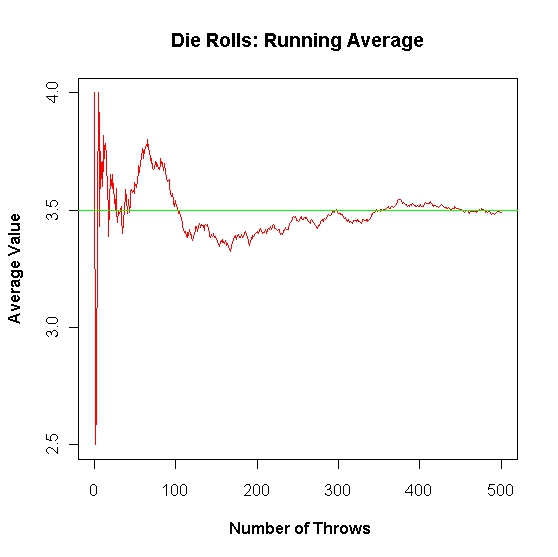
\includegraphics[scale=0.4]{images/2BDieMean}
		\end{center}
		
	}
	%--------------------------------------------------------%
	{
		\textbf{Thought Experiment}
		
		\begin{itemize}
			\item Suppose you roll a die 100 times. You record the outcome for each roll, and compute the sum of the 100 rolls at the end.
			\item What sum do you expect to end up with?
			\item The lowest sum that is mathematically possible is 100. The highest is 600. To get either of these, you would have to roll the same number (either 1 or 6) 100 times in a row. Very unlikely ( but not impossible).
			\item Instead you would expect to end up half way between 100 and 600, i.e. 350.
			\item Every roll of a die should be worth 3.5 on average to your overall score.
		\end{itemize}
	}
	%--------------------------------------------------------%
	
	{
		
		\textbf{Expected Value for Discrete Random Variables}
		
		\begin{itemize}
			\item The expected value of a discrete random variable $X$ is symbolized by E(X).
			
			\item If X is a discrete random variable with possible values $\{ x_1, x_2, x_3,\ldots , x_n\}$, and $p(x_i)$ denotes $P(X = x_i)$, then the expected value of $X$ is defined by:
			
			\[
			E(X) = \sum x_i \times p(x_i)
			\]
			
			where the elements are summed over all values of the random variable $X$.
			
		\end{itemize}
		
		\textbf{Remark: } Expected values for continuous random variables are defined, but are not part of this module.
	}
	%--------------------------------------------------------%
	{
		\textbf{Expected Value for Discrete Random Variables}
		When a die is thrown, each of the possible sides 1, 2, 3, 4, 5, 6 (i.e. the $x_i$ 's) has a
		probability of 1/6 (the $p(x_i)$ s) of showing.
		\\ \bigskip
		The expected value of the face showing is therefore:
		
		\[E(X) = (1 \times 1/6) + (2 \times 1/6) + (3 \times 1/6) + (4 \times 1/6) + (5 \times 1/6) + (6 \times 1/6)\]
		
		\[E(X) = 21/6 = 3.5 \]
		\bigskip
		Notice that, in this case, $E(X)$ is $3.5$, which is not a possible value of X.
		
		
	}
	%--------------------------------------------------------%
	{
		\textbf{Expected Value for Discrete Random Variables}
		
		Suppose we are playing a game where the points scored in each round are the square of the value shown by the die?
		What is expected value of the score for each round.
		\\ \bigskip
		As we have defined a random variable $X$ to represent the number shown by each roll, we will define another $X^2$ to represent the points accrued by each roll.
		\\ \bigskip
		The expected value can be computed as follows:
		\[
		E(X^2) = \sum (x_i^2) \times p(x_i)
		\]
	}
	%--------------------------------------------------------%
	{
		\textbf{Expected Value for Discrete Random Variables}
		The expected value of the points is therefore:
		
		\[E(X^2) = (1^2 \times 1/6) + (2^2 \times 1/6) + (3^2 \times 1/6) + (4^2 \times 1/6) + (5^2 \times 1/6) + (6^2 \times 1/6)\]
		
		\[E(X^2) = 91/6 = 15.16 \]
		
		
	}
	
	
	
	
	
	
	%--------------------------------------------------------%
	{
		\textbf{Variance of a Discrete Random Variable}
		We may require to know the variance of the random variable.
		
		The variance of the random variable X, denoted $V(X)$, is defined to be:
		\[ V(X) = E(X^2) - E(X)^2 \]
		where $E(X)$ is the expected value of the random variable X.
	}
	
	
	%--------------------------------------------------------%
	{
		\textbf{Variance of a Discrete Random Variable}
		Compute the variance for outcomes of the throws of a die, using
		\[ V(X) = E(X^2) - E(X)^2 \].
		
		We know that \begin{itemize} \item $E(X) = 21/6$ , so  $E(X)^2 = 441/36$. \\
			
			\item $E(X^2)  = 91/6  = 546/36$
			
			\item Therefore $V(X) = 546/36 - 441/36 = 105/36 = 2.91$
		\end{itemize}
		
	}	
\section{Expected Values of Random Variables}

If the random variable $Z$ has a distribution which is standard normal, show that the expected value of $e^{sZ}$ is given as follows:

\[E(e^{sZ})  =  e^{\frac{s^2}{2}}\] 


\begin{itemize}
	\item In general, the expected value is computed using this formula
	{
		
		\[ E(X) =  \int_{-\infty}^{\infty}  x \times f(x) dx   \]
	}
	\item The expected value of a \textbf{\textit{transformed}} random variable is computed using this formula
	{
		
		\[ E( tf(X) ) =  \int_{-\infty}^{\infty}  tf(x) \times f(x) dx   \]
	}
	
	\item 
	The probability density function for the standard normal distribution is
	
	
	%	\[f(x, \mu, \sigma) = \frac{1}{\sigma\sqrt{2\pi}} e^{ -\frac{(x-\mu)^2}{2\sigma^2} }\]}
	\item 
	The probability density function for the standard normal distribution is
	
	
	\[f(z) = f(x, \mu= 0, \sigma=1) = \frac{1}{\sqrt{2\pi}} e^{ -{x \over 2}^2 }\]
	
\end{itemize}




{
	
	\[ E( e^{sZ} ) =  \int_{-\infty}^{\infty}  e^{sx} \;\times\; \frac{1}{\sqrt{2\pi}} \;e^{ -{x \over 2}^2 }\]
	
	
	\[ E( e^{sZ} ) =  \frac{1}{\sqrt{2\pi}} \int_{-\infty}^{\infty}   e^{ \big[sx-\frac{(x)^2}{2} \big]} dx   \]
	
	\[ E( e^{sZ} ) =  e^{{s^2\over 2}} \; \times\; \frac{1}{\sqrt{2\pi}} \int_{-\infty}^{\infty} e^{ \big[-\frac{(x-s)^2}{2} \big]} dx   \]
}



\textbf{Mathematical Identity}
\begin{itemize}
	\item Proven in a separate video
\end{itemize}
{
	
	\[\int_{-\infty}^{\infty} e^{-{y\over 2}^2}dy  = \sqrt{2\pi}\]
	
}




{
	
	\[ E( e^{sZ} ) =  e^{{s^2\over 2}} \; \times\; \frac{1}{\sqrt{2\pi}} \int_{-\infty}^{\infty} e^{ \big[-\frac{(x-s)^2}{2} \big]} dx \]
	
	
	\[ E( e^{sZ} ) =  e^{{s^2\over 2}} \; \times\; \frac{1}{\sqrt{2\pi}} \big[\sqrt{2\pi} \big] \]
}



	\chapter{Calculus for Random Variables}
	
	\section{Expected Values of Random Variables}
	
	If the random variable $Z$ has a distribution which is standard normal, show that the expected value of $e^{sZ}$ is given as follows:
	
	\[E(e^{sZ})  =  e^{\frac{s^2}{2}}\] 
	
	
	\begin{itemize}
		\item In general, the expected value is computed using this formula
		{
			
			\[ E(X) =  \int_{-\infty}^{\infty}  x \times f(x) dx   \]
		}
		\item The expected value of a \textbf{\textit{transformed}} random variable is computed using this formula
		{
			
			\[ E( tf(X) ) =  \int_{-\infty}^{\infty}  tf(x) \times f(x) dx   \]
		}
		
		\item 
		The probability density function for the standard normal distribution is
		
		
		%	\[f(x, \mu, \sigma) = \frac{1}{\sigma\sqrt{2\pi}} e^{ -\frac{(x-\mu)^2}{2\sigma^2} }\]}
		\item 
		The probability density function for the standard normal distribution is
		
		
		\[f(z) = f(x, \mu= 0, \sigma=1) = \frac{1}{\sqrt{2\pi}} e^{ -{x \over 2}^2 }\]
		
	\end{itemize}
	
	
	
	
	{
		
		\[ E( e^{sZ} ) =  \int_{-\infty}^{\infty}  e^{sx} \;\times\; \frac{1}{\sqrt{2\pi}} \;e^{ -{x \over 2}^2 }\]
		
		
		\[ E( e^{sZ} ) =  \frac{1}{\sqrt{2\pi}} \int_{-\infty}^{\infty}   e^{ \big[sx-\frac{(x)^2}{2} \big]} dx   \]
		
		\[ E( e^{sZ} ) =  e^{{s^2\over 2}} \; \times\; \frac{1}{\sqrt{2\pi}} \int_{-\infty}^{\infty} e^{ \big[-\frac{(x-s)^2}{2} \big]} dx   \]
	}
	
	
	
	\textbf{Mathematical Identity}
	\begin{itemize}
		\item Proven in a separate video
	\end{itemize}
	{
		
		\[\int_{-\infty}^{\infty} e^{-{y\over 2}^2}dy  = \sqrt{2\pi}\]
		
	}
	
	
	
	
	{
		
		\[ E( e^{sZ} ) =  e^{{s^2\over 2}} \; \times\; \frac{1}{\sqrt{2\pi}} \int_{-\infty}^{\infty} e^{ \big[-\frac{(x-s)^2}{2} \big]} dx \]
		
		
		\[ E( e^{sZ} ) =  e^{{s^2\over 2}} \; \times\; \frac{1}{\sqrt{2\pi}} \big[\sqrt{2\pi} \big] \]
	}
	
	

\end{document}